\documentclass[tikz,border=8pt]{standalone}
% Shared look for every TikZ diagram. Load with \input{../../tools/tikz-style.tex}
\usepackage[T1]{fontenc}
\usepackage{lmodern}
\renewcommand{\sfdefault}{lmr}  % diagrams use the same serif as the text
\usetikzlibrary{arrows.meta, positioning, shapes.geometric, calc, fit, backgrounds}
\definecolor{cblue}{HTML}{4C78A8}
\definecolor{corange}{HTML}{F58518}
\definecolor{cgreen}{HTML}{54A24B}
\definecolor{cred}{HTML}{E45756}
\definecolor{cpurple}{HTML}{B279A2}
\definecolor{cgrey}{HTML}{6B6B6B}
\tikzset{
  every picture/.style={font=\sffamily, line width=1.2pt},
  box/.style={draw=#1, fill=#1!12, rounded corners=4pt, align=center, inner sep=7pt, minimum height=1.1cm},
  box/.default=cgrey,
  arrow/.style={-{Stealth[length=3mm]}, draw=cgrey, line width=1.4pt},
  title/.style={font=\sffamily\bfseries\Large},
  note/.style={font=\sffamily\small, text=cgrey, align=center},
}
\AtBeginDocument{\hyphenpenalty=10000 \exhyphenpenalty=10000}

\begin{document}
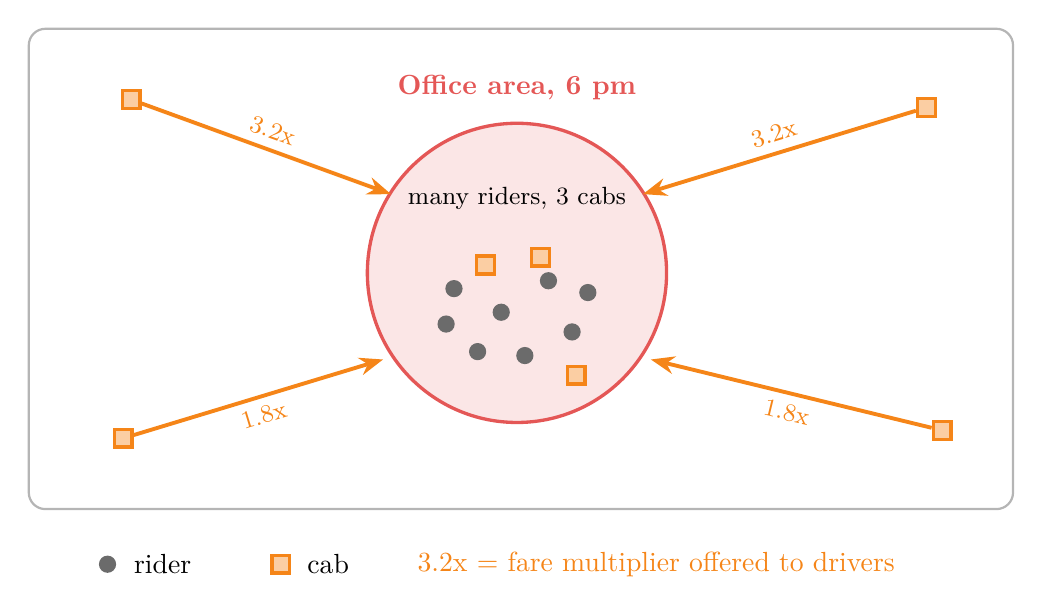
\begin{tikzpicture}
  % city area
  \draw[cgrey!50, rounded corners=6pt, line width=0.8pt] (-1,-0.6) rectangle (11.5,5.5);
  % hot zone
  \node[draw=cred, fill=cred!15, circle, minimum size=3.8cm, align=center] (hot) at (5.2,2.4) {};
  \node[font=\bfseries, text=cred] at (5.2,4.75) {Office area, 6 pm};
  \node[align=center, font=\small] at (5.2,3.35) {many riders, 3 cabs};
  \foreach \p in {(4.4,2.2),(5.0,1.9),(5.6,2.3),(4.7,1.4),(5.3,1.35),(5.9,1.65),(4.3,1.75),(6.1,2.15)}
    \node[fill=cgrey, circle, inner sep=2.2pt] at \p {};
  \foreach \p in {(4.8,2.5),(5.5,2.6),(5.95,1.1)}
    \node[draw=corange, fill=corange!40, rectangle, inner sep=3.2pt] at \p {};
  % drivers outside
  \node[draw=corange, fill=corange!40, rectangle, inner sep=3.2pt] (d1) at (0.3,4.6) {};
  \node[draw=corange, fill=corange!40, rectangle, inner sep=3.2pt] (d2) at (0.2,0.3) {};
  \node[draw=corange, fill=corange!40, rectangle, inner sep=3.2pt] (d3) at (10.4,4.5) {};
  \node[draw=corange, fill=corange!40, rectangle, inner sep=3.2pt] (d4) at (10.6,0.4) {};
  \draw[arrow, corange] (d1) -- node[note, above, sloped, text=corange] {3.2x} (3.6,3.4);
  \draw[arrow, corange] (d2) -- node[note, below, sloped, text=corange] {1.8x} (3.5,1.3);
  \draw[arrow, corange] (d3) -- node[note, above, sloped, text=corange] {3.2x} (6.8,3.4);
  \draw[arrow, corange] (d4) -- node[note, below, sloped, text=corange] {1.8x} (6.9,1.3);
  % legend
  \node[fill=cgrey, circle, inner sep=2.2pt] at (0,-1.3) {};
  \node[anchor=west] at (0.2,-1.3) {rider};
  \node[draw=corange, fill=corange!40, rectangle, inner sep=3.2pt] at (2.2,-1.3) {};
  \node[anchor=west] at (2.4,-1.3) {cab};
  \node[anchor=west, text=corange] at (3.8,-1.3) {3.2x = fare multiplier offered to drivers};
\end{tikzpicture}
\end{document}
